\documentclass[11pt]{article}

\usepackage[utf8]{inputenc}
\usepackage[english]{babel}

\usepackage{mathtools}

\usepackage{setspace}
\onehalfspacing

\usepackage{amsfonts}
\usepackage{amsmath}
\usepackage{amsthm}
\usepackage{indentfirst}
\newtheorem{theorem}{Theorem}
\newtheorem{lemma}{Lemma}
\newtheorem{example}{Example}
\newtheorem{definition}{Definition}
\newtheorem{remark}{Remark}
\newtheorem{corollary}{Corollary}

\newtheorem*{theorem*}{Theorem}
\newtheorem*{lemma*}{Lemma}
\newtheorem*{example*}{Example}
\newtheorem*{definition*}{Definition}
\newtheorem*{remark*}{Remark}
\newtheorem*{corollary*}{Corollary}

%\usepackage{booktabs, caption, graphicx, float}
%\usepackage{subcaption}
%\captionsetup{tableposition=top,figureposition=bottom,font=small}

\usepackage{comment}
\usepackage{multirow}
\usepackage{array}

\newcolumntype{C}[1]{>{\centering\let\newline\\\arraybackslash\hspace{0pt}}m{#1}}
\DeclarePairedDelimiter\floor{\lfloor}{\rfloor}

\usepackage[hidelinks]{hyperref}

\usepackage{geometry}
\geometry{a4paper, top=3cm,bottom=3cm,left=3cm,right=3cm,%
	heightrounded}
\usepackage{upgreek}
\usepackage{xparse}
\usepackage{listings}
\NewDocumentCommand{\codeword}{v}{%
	\texttt{\textcolor{black}{#1}}%
}

\newcommand{\prepos}[3]{${}_{\mathbf{#2}}{\mathbf{#1}}_{#3}$}
\newcommand{\preposm}[3]{{}_{\mathbf{#2}}{\mathbf{#1}}_{#3}}


%Dummy text
\usepackage{lipsum}

%Changing headers and footers
\usepackage{fancyhdr}
\pagestyle{fancy}
\fancyhf{}
\rhead{\textit{\thepage}}
\lhead{\textit{Joint Space Motion Control Lab}}

%For inserting the code
\usepackage{fancyvrb}

%For bold math symbols
\usepackage{bm}

%For multicolumns
\usepackage{multicol}

% Norm and abs delimiter
\usepackage{mathtools}
\DeclarePairedDelimiter{\abs}{\lvert}{\rvert}
\DeclarePairedDelimiterX{\norm}[1]{\lVert}{\rVert}{#1}

\setcounter{section}{-1}

% Argmin/Argmax
\DeclareMathOperator*{\argmax}{argmax}
\DeclareMathOperator*{\argmin}{argmin}

% Enumerate
\usepackage{enumitem}

% Code
\usepackage{algorithm}
\usepackage[noend]{algpseudocode}
\usepackage{etoolbox}

% Longtable
\usepackage{longtable}

% SI units
\usepackage{siunitx}
\sisetup{output-exponent-marker=\ensuremath{\mathrm{e}}}

% Colours in equations
\usepackage{xcolor}

\newcommand{\Rnum}{\mathbb{R}} % Symbol fo the real numbers set
\newcommand{\mat}[1]{\ensuremath{\begin{bmatrix}#1\end{bmatrix}}}	% matrix
\newcommand{\myparagraph}[1]{\paragraph{#1}\mbox{}\\}


\title{LAB 2: Joint Space Motion Control Lab: Control of a 6-DoF Serial Manipulator}
\author{Michele Focchi and Matteo Saveriano}
\date{}

\begin{document}
	\maketitle
	\noindent
	The goals of this assignment are:
	\begin{itemize}
		\item learning the basic procedure to design a motion controller in the joint space for a manipulator in free-motion (i.e. not in contact)
		\item analyze the advantage/disadvantage of decentralized/ centralized approaches (i.e. feedback linearization)
		\item implement the interaction with the environment with a compliant contact model	 
	\end{itemize}
	
	\noindent
	Tools that we are going to be using in this lab (all open-source):
	\begin{itemize}
		\item Python programming (2.7/3.5)\footnote{https://docs.python.org/}
		\item Robot Operating System (ROS)\footnote{https://www.ros.org/}
		\item Pinocchio Library for Rigid Body Dynamics Algorithms\footnote{https://github.com/stack-of-tasks/pinocchio}
		\item Locosim\footnote{https://github.com/mfocchi/locosim}
	\end{itemize}
	%
	%
	%\noindent
	In this assignment we will  design the controller for a 6-DoF anthropomorphic robot manipulator (UR5, see  Fig.~\ref{fig:UR5}). We have already seen how to simulate a UR4 robot without any actuation torques. Now we want to write a controller that generates the actuation torques in order to track a desired reference trajectory. First, we will design some references defined at the joint level. Then, we will design several control laws with increasing complexity evaluating their impact on the accuracy and the tracking errors at the joints. The loop will be always closed at the joint level.  
 
 %
 \begin{figure}[bht]
 	\centering
 	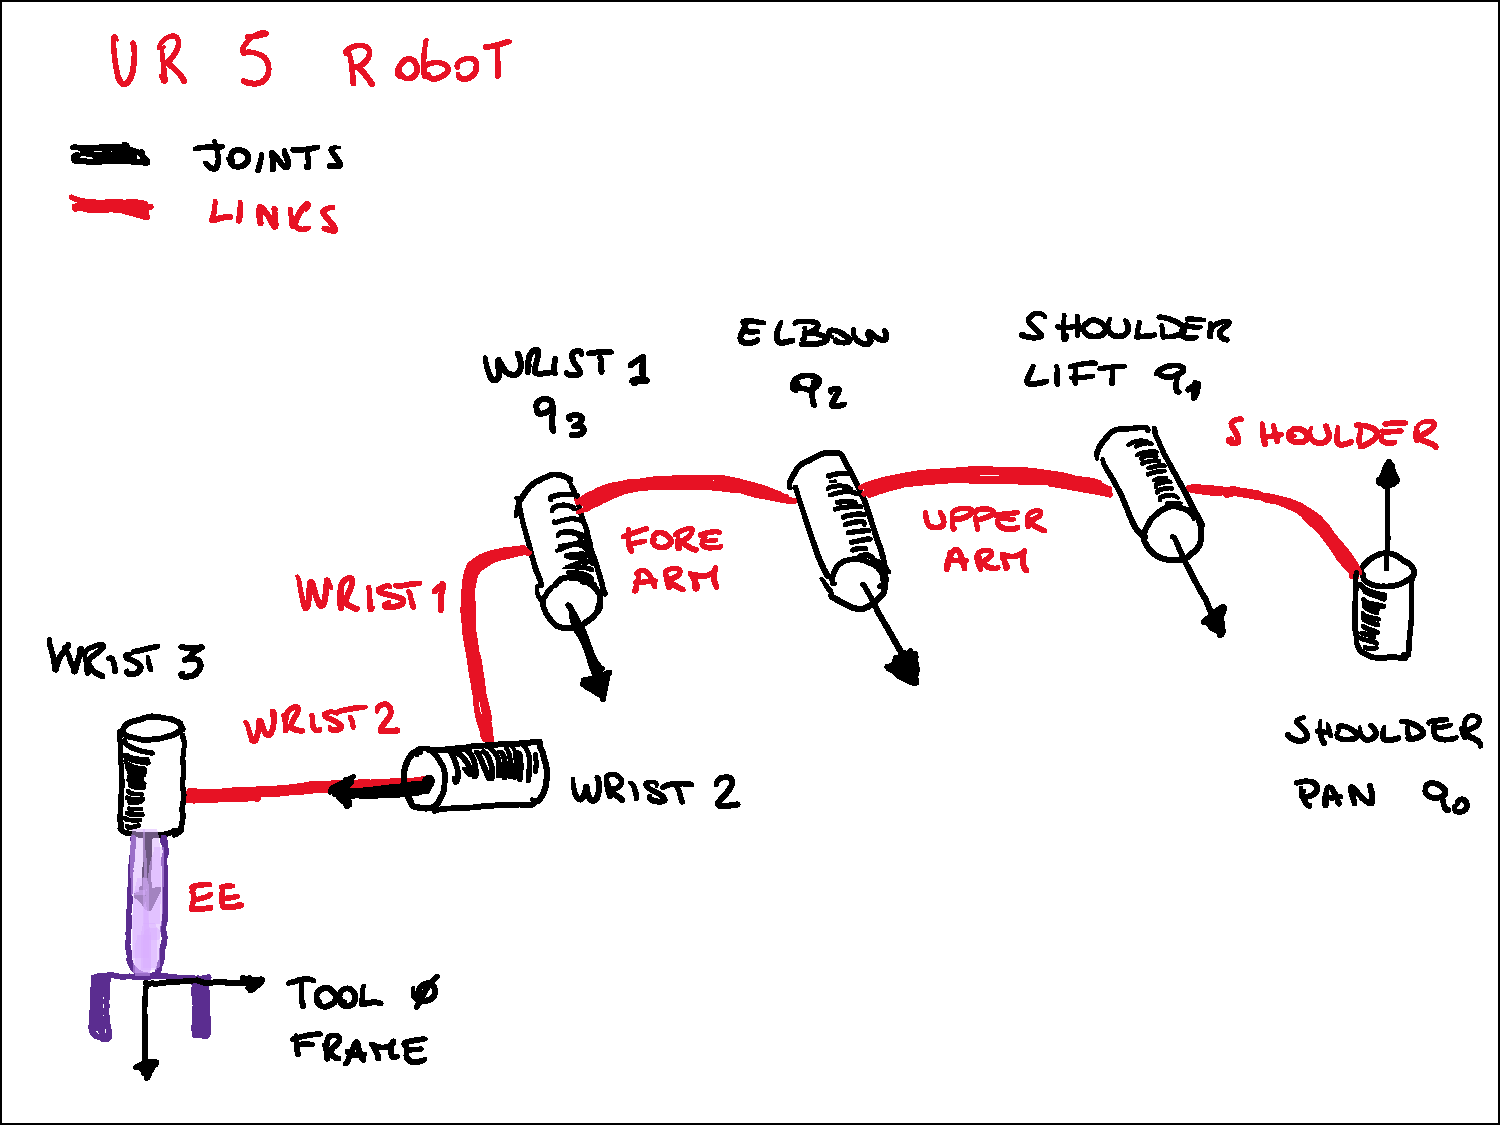
\includegraphics[width=8cm]{pics/ur5_Robot.pdf}
 	\caption{Kinematics of the UR5 Robot.}
 	\label{fig:UR5}
 \end{figure}

\section{Preliminaries}

Remember to recompile the framework after any update:

\begin{verbatim}
cd ~/ros_ws
catkin_make install
\end{verbatim}

To test the RVIZ visualization and have a grasp on the kinematic of the UR5 robot, try to move the joints with the sliders, running:
%
\begin{verbatim}
roslaunch ros_impedance_controller visualize.launch robot_name:=ur5 
\end{verbatim}

\section{Decentralized control (Lecture G0)}

\noindent
\textbf{1.1 - Sinusoidal Reference generation:}
 Generate a sinusoidal reference for the $2^{nd}$ (Shoulder Lift) and $5^{th}$  (Wrist 2) joint with frequency 1.0 $Hz$ and 1.5 $Hz$ and amplitude 0.2$rad$ and 0.4 $rad$, respectively,  starting from their initial configurations in $q_0$. Keep the other joints at $q_0$. After 4.0 $s$ stop the sine and give a constant reference during  1.0 $s$. Note that you need to generate also consistent references for velocity and acceleration.

\quad

\noindent
\textbf{1.2 - Step Reference generation:} generate a -0.4 $rad$, 0.5 $rad$ step reference change step at $t= 2.0s$ for the $2^{nd}$ (Shoulder Lift) and $5^{th}$  (Wrist 2) joint, respectively, starting from their initial configuration in $q_0$. Keep the other joints at $q_0$.

\quad

\noindent
\textbf{1.3 - Joint PD control:}
Implement a Joint $PD$ control law with proportional $K_p$ = 300 $Nm/rad$ and derivative $K_d$ = 20 $Nms/rad$ gains for all the joints. Use the step reference generated in (1.2). Plot the reference and the actual joint position for all the joints and see that a tracking error is present both during the transient and at steady-state. Explain why there is almost no tracking error in the $5^{th}$ joint. % because Kp for the inertia is very stiff
Is there any overshoot in the $2^{nd}$ joint? 

\quad

\noindent 
\textbf{1.4 - Joint PD control – high gains:}
Using the same PD control law increase the gains (set them in the \codeword{ex_2_conf.py}) to $K_p$ = 600 $Nm/rad$ and $K_d$ = 30 $Nms/rad$.  Use the step reference generated in (1.2). See that the tracking 
error on $2^{nd}$ joint is reduced of almost half (i.e. from 0.2 to 0.1 $rad$ on $2^{nd}$ joint). Play around with the value of $K_d$. See that the system becomes unstable if you 
increase too much $K_d$ (e.g. for $K_d>33$)  because the phase margin is going to zero. Now remember that the digital implementation of the controller introduces delays. Try to reduce the sampling time $dt$ to 0.0001 $s$ and see what is the maximum value of $K_d$ you can set (i.e. 300) before the robot gets unstable (use sinusoidal reference).

\quad

\noindent
\textbf{1.5 - Joint PD control critical damping:}
Until now, we did not take into account the fact that the inertia changes with the joint configuration, therefore a fixed value of $K_d$ is not suitable to obtain 
the same transient shape at different joint configurations. Set the proportional gain back to a constant value $K_p$ = 300 $Nm/rad$, but update the derivative gain 
$K_d$ at each loop in order to achieve a \textit{critical damping} for all  joints. We explained that the PD control can be seen as equivalent to a $2{nd}$ order 
spring-mass-damper system with stiffness $K_p$ and damping $K_d$. 
Therefore you can use the inertia seen by each joint (i.e. the elements $m_{i,i}$ on the diagonal 
of the inertia matrix) and set $K_{d,i} = 2\sqrt{K_{p,i} m_{i,i}}$ to achieve a critical damping response (natural damping ratio $\zeta = 1$). Use the step 
generated in (1.2) as reference, see that the overshoot disappeared in $2^{nd}$ joint but there is a steady-state error due to gravity. Using the sinusoidal 
reference in (1.1) % can add 0.8 1.0 -3.14 to 3rd joint too
check that the variation in the damping of the $2^{nd}$ joint is much bigger that for the $5^{th}$ joint, because the inertia seen by a joint  is dependent on the motion of all the subsequent joints and joints that are more proximal to the base are moving the inertia of more links after them.
Set the following parameters in the sine reference to create a motion with bigger inertia variation and better visualize this phenomena:


\begin{verbatim}
amp = np.array([ 0.0, 0.4, 0.8, 0.0, 0.4, 0.0])    
phi = np.array([ 0.0, 0.0, 3.14, 0.0, 0.0, 0.0])      
freq = np.array([ 0.0, 1.0, 1.0, 0.0, 1.5, 0.0])    
\end{verbatim}


\quad

\noindent
\textbf{1.6 - Joint PD control + Gravity Compensation:}
Now, let's add a gravity compensation term to compensate gravity forces at the joints. 
Compute this term with Pinocchio library at each loop and notice that it is changing with the configuration. 
Give the step reference generated in (1.2) as input to the closed loop system. 
Check there is no longer a  tracking error at steady-state but it is still present during the transient. What are these error due to?
Check also the tracking with the sinusoidal reference generated in (1.1).

\quad

\noindent
\textbf{1.7 - Joint  PD + gravity + Feed-Forward term:}
At this point, let's see the impact of adding a feed-forward term to the PD control (advice: use the inertia seen by each joint). Note that you should use desired joint values $q^d$ to compute the inertia in a pure feed-forward approach. This approach will improve the tracking error for a time-varying reference signal, so use the sinusoidal reference generated in (1.1).  See that the tracking error is significantly improved for the joints that are moving. However, if you look at the plot of the joints that are supposed to stay still, there are still disturbances coming from the motion of the moving joints. These disturbances are  due to the \textit{inertial couplings} and cannot be dealt with a \textit{decentralized} approach.

\quad

\section{Centralized control (Lecture G1)}

\noindent
\textbf{2.1 - Inverse Dynamics (Computed Torque):}
To effectively compensate for the inertial couplings, we can compensate them by 
linearizing the (non linear) dynamics of the robot via a state feedback called feed-back linearization. 
This approach, that is valid for any non linear system, for articulated robots takes the name of \textit{Inverse Dynamics}(Computed Torque). 
The intuition is based on cancelling nonlinear terms and decoupling the dynamics of each link.
The basic idea of feedback linearization is to construct a transformation which exactly linearizes the
nonlinear system after a suitable state space change of coordinates (e.g the new input to the system becomes $v$).
 One can then design a second stage (or outer-loop) control in the new coordinates to satisfy the traditional control design specifications such as tracking,
disturbance rejection, etc.
Implement the inverse dynamics  (computed Torque) algorithm at the joint space. Keep the same $K_p$, $K_d$ gains as in (1.3) and add a Feed-forward acceleration term $\ddot{q}^d$. 

\begin{equation*}
u = M(q) (\ddot{q}^d + K_{p} (q^d  - q) + K_{d} (\dot{q}^d  - \dot{q}) + h(q,\dot{q}))
\end{equation*}

Observe that the tracking errors  now are  always zero also for the joints that are not moving, 
the inertial couplings are properly compensated. 
Now plot also the tracking of joint velocity. Why there is a tracking error at the beginning? 

\quad

\noindent
\textbf{ 2.2 - Inverse Dynamics (Computed Torque) – initial velocity:}
Change the initial value of the joint velocities, to be consistent with the initial reference velocity, and see the tracking error is zero also at the beginning, for all the joints. 

\quad

\noindent
\textbf{ 2.3 - Inverse Dynamics (Computed Torque) – low gains:}
Inverse dynamics completely decouple the system into a set of pure double integrators on the new input $v$:

\begin{equation*}
\ddot{q}_i = v_i  \quad i = 1, \dots, n
\end{equation*}

then the transient of each joint can be tuned separately for each joint setting the gains in the respective  control law:

\begin{equation*}
v_i  = \ddot{q}^d_i + K_{p,i} (q^d_i  - q_i) + K_{d,i} (\dot{q}^d_i  - \dot{q}_i) \quad i = 1, \dots, n
\end{equation*}

Note that to achieve critical damping how you need to set $k_{d,i} = 2\sqrt{K_{p,i}}$ because inertia is the one of an \textit{unitary} mass.
In absence of external disturbances, verify that the tracking is perfect, 
even if you decrease the $K_p$, $K_d$ gains.  Reduce the $K_p$ to 1/$5^th$ ($K_p = 60$) and observe the tracking is still perfect both for the joints in motion and not in motion. This is different with respect to a decentralized approach where, if we decrease the gains,  the influence of the inertial couplings becomes more  prominent and, hence, apparent.   

\quad

\noindent
\textbf{2.4 - Inverse Dynamics (Computed Torque) – External force:} 
Now try to add an external (3D) force applied at the end-effector $F_{ext} =[0,0,50] N$ (i.e. along the $Z$ direction),
starting at $t= 3s$ (hint: add  $J^TF_{ext}$ to $\tau$). Check than now tracking errors appear on all the joints due to the external disturbance that affect all the joints though  $J^T$. Keep the  reference  constant to $q_0$ to better visualize this. Note that the joint most affected is the elbow.
Restore $K_p$ back tp $300$ and see that the tracking error reduces to 1/$5^th$ because we have linearized the system, and therefore to increasing the gain will reduce the error of the same amount. 
Play with different values of the  $K_p$ gain showing that with higher values of the gain the error is reduced.

\quad

\noindent
\textbf{2.5 - Inverse Dynamics (Computed Torque) – uncertainty in the cancellation:}
%
In real systems we always have uncertainty in our model due to modeling 
limitations of  CAD  drawing, non idealities, unmodeled dynamics, compliance of the structure, etc.
This means that the matrix $\hat{M}$ and $\hat{h}$ we use in the inverse dynamics will be slightly different from the real ones ${M}$ and ${h}$, leading to a not perfect cancellation. Add a 10\%   parametric variation (uncertainty) to scale the elements of $M$ and $h$  to obtain $\hat{M}$ and $\hat{h}$  to be used in the inverse dynamics scheme. % or use matrix norm: np.linalg.norm(M)*0.1*np.random.rand(6, 6) or uncertainty = (1.0 + 0.1*np.random.rand())
Evaluate the degradation in tracking performances due to a not perfect cancellation, with the sinusoidal reference (1.1). Remember to remove the external force that is not needed for this exercise.

\quad

\noindent
\textbf{ 2.6 - Inverse Dynamics (Desired states):}
Now remove  the parametric scaling from  $M$ and $h$  but use the desired values of the states $\dot{q}^d$ , $q^d$  instead of 
the actual values $\dot{q}$ , $q$ to compute them. During the transient some coupling start to appear because there is always a small difference between $q^d$ and $q$, so a not prefect cancellation. This worsen significantly at the end of the sinusoids when there is a not smooth derivative of the reference that causes a bigger tracking error.
 
\quad

\noindent 
\textbf{ 2.7 - Unilateral Compliant contact:} 
To complete this lab, we want to consider an interaction of the robot with the environment happening at the end-effector. 
Model the contact using a compliant model with linear  springs $K_{env}\in \Rnum^{3 \times 3}$ and dampers $D_{env}\in \Rnum^{3 \times 3}$  and insert the resulting contact force $F_{env} \in R^3$ into the free-motion dynamics via the $J^T$. Consider the contact \textit{unilateral} and for now allow the force to be generated only along the Z direction (contact normal).
Note you need also to compute the end-effector velocity for the damping term (i.e. use $\dot{p} = J\dot{q}$).

\begin{equation*}
\begin{cases}
	F_{env} = n n^T (K_{env}(p_0 - p) - D_{env} \dot{p}) \quad &\text{   if}\quad n^T(p_0 -p ) >0 \\ 
	F_{env} = 0     \quad &\text{if}\quad n^T(p_0 -p ) <0
\end{cases}
\end{equation*}

The approach we used (\textit{forward Euler}) to integrate the acceleration is not ideal for stiff dynamic equations. Try to increase the stiffness $K_{env}$ till the limit where the integration scheme becomes unstable (i.e. $D_{env} = eye(3)100000 Ns/m$).
Notice that the end-effector is  sliding at the contact in the horizontal direction because we projected $F_{env}$ along the contact normal.
try to use the full 3D force computed by the contact model:
%
\begin{equation*}
\begin{cases}
F_{env} = K_{env}(p_0 - p) - D_{env} \dot{p} \quad &\text{   if}\quad n^T(p_0 -p ) >0 \\ 
F_{env} = 0     \quad &\text{if}\quad n^T(p_0 -p ) <0
\end{cases}
\end{equation*}
%
Note that now you need also to sample the position $p_0$ at the contact to keep memory of the horizontal components.
Notice that the contact does not move in the horizontal direction, like if the end-effector was clamped on the floor and internal motions appear on the joints that comply with the contact constraint. 

\quad

\noindent
\textbf{ 2.7 - Coulomb friction:} 
However, our contact point is not really ``glued" to the ground and there is a limit on the tangential force the floor can apply,  
beyond which the end-effector starts to slip (Coulomb friction model).  This tangential force depends on the friction coefficient $\mu$ (that on its behalf it depends on the nature of both contacting surfaces). Incorporate a friction cone constraints (see. Fig \ref{fig:fcone}) by clamping  appropriately the tangential forces using  a friction coefficient $\mu = 1.0$:

\begin{equation*}
\begin{cases}
F_{env, x} = \mu F_{env, z}  \quad &\text{   if}\quad F_{env, x} \geq \mu F_{env, z} \\ 
F_{env, x} = -\mu F_{env, z}  \quad &\text{   if}\quad F_{env, x} \leq -\mu F_{env, z} \\ 
F_{env, y} = \mu F_{env, z}  \quad &\text{   if}\quad F_{env, y} \geq \mu F_{env, z} \\ 
F_{env, y} = -\mu F_{env, z}  \quad &\text{   if}\quad F_{env, y} \leq -\mu F_{env, z} \\ 
\end{cases}
\end{equation*}
%
 \begin{figure}[bht]
 	\centering
 	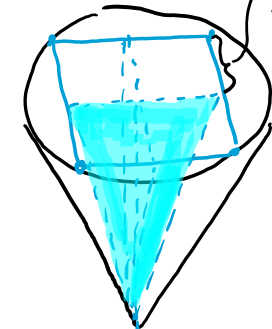
\includegraphics[width=2.5cm]{pics/fcone2.png}
 	\caption{Pyramid (linear) approximation of the friction cone.}
 	\label{fig:fcone}
 \end{figure}
Now simulate and slow down the motion if it is necessary using the slow factor in the configuration file. 
Plot also the shape of the cone wth the \codeword{add_cone()} function and  see that the force at the end-effector is violating friction constraints only at the very end and no slippage occurs. This means that, for $\mu = 1.0$, the friction forces from the floor are still high enough to keep the contact in the horizontal direction.  Reduce the friction coefficient to $\mu = 0.05$ and observe that a slippage starts to occur and the forces are limited inside the cone.  
% 
\end{document}